
\subsubsection{25.10.14}

\begin{enumerate}
	\item Время начала и окончания собрания:
	16:00 - 20:00
	\item Цели собрания:
	\begin{enumerate}
	  \item Спроектировать и собрать механизм захвата передвижных корзин.
	  
    \end{enumerate}
    
	\item Проделанная работа:
	\begin{enumerate}
	  \item Было рассмотрено 2 варианта исполнения механизма захвата корзин (далее он будет называться МЗК):
	  \begin{enumerate}
	    \item Сервопривод, к которому прикреплен один конец балки, и при вращении сервопривода балка поворачивается и опускается.
	    
	    \item К заднему краю корпуса робота прикреплена мебельная рейка, соединенная с сервоприводом через леску и опускающаяся при его вращении.
	    
	    \begin{figure}[H]
	    	\begin{minipage}[h]{0.2\linewidth}
	    		\center   
	    	\end{minipage}
	    	\begin{minipage}[h]{0.6\linewidth}
	    		\center{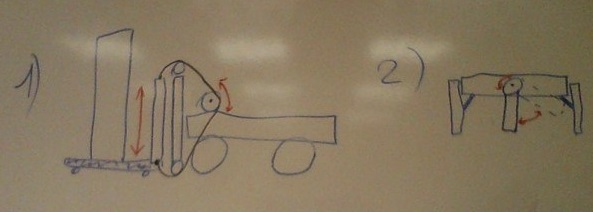
\includegraphics[scale=0.55]{days/25.10.14/images/01}}
	    		\caption{Идеи для механизма захвата передвижных корзин 1)Рейка 2)Сервопривод}
	    	\end{minipage}
	    \end{figure}
	    
      \end{enumerate}
      \item Предпочтение было отдано второму в силу его большей компактности.
      
      \item Мебельная рейка была распилена для уменьшения ее длины.
      
      \begin{figure}[H]
      	\begin{minipage}[h]{0.2\linewidth}
      		\center   
      	\end{minipage}
      	\begin{minipage}[h]{0.6\linewidth}
      		\center{
\includegraphics[scale=0.24]{days/25.10.14/images/02}}
      		\caption{Укороченная мебельная рейка \newline (заштрихована отпиленная часть)}
      	\end{minipage}
      \end{figure}
      
      \item На рейке размечены места для сверления отверстий под крепеж. Сам отверстия просверлены не были ввиду отсутствия на занятии дрели.
      
    \end{enumerate}
    
	\item Итоги собрания: 
	\begin{enumerate}
	  \item МЗК спроектирован, но не установлен.
      
    \end{enumerate}
    
	\item Задачи для последующих собраний:
	\begin{enumerate}
	  \item Закончить создание МЗК.
	  
    \end{enumerate}     
\end{enumerate}
\fillpage
